\chapter{Wstęp}

\section{Wprowadzenie}

Wstępne koncepcje systemów realizujących aktywne tłumienie hałasu 
(ANC, ang. \textit{Active noise control})
zaczęły pojawiać się już w latach 30. XX wieku, jednak
z powodu braku odpowiednich narzędzi technologicznych pozwalających
na praktyczną implementację rozwiązania w tamtych czasach, 
znaczące postępy zaczęto obserwować dopiero w latach 80. 
i 90. XX wieku, kiedy raptowny rozwój technologiczny
umożliwił projektowane coraz to dokładniejszych i stabilniejszych układów 
automatyki \cite{bib:kuo_morgan}. Powodem takiego przebiegu wydarzeń był wyłaniający 
się zza horyzontu początek epoki cyfrowej, potwierdzającej prorocze słowa 
Claude'a Shannona o potędze kodu binarnego, z użyciem którego można opisać i 
wpływać na otaczający nas świat z dużą precyzją i elastycznością, nieosiągalną 
wcześniej w rozwiązaniach opartych jedynie na technice analogowej.

\par Zastosowanie układów cyfrowych w systemach ANC
umożliwiło zatem ich szersze wykorzystanie w praktyce. Zaskutkowało to 
gwałtownym rozwojem omawianej tematyki. ANC znalazło swoje 
zastosowanie w redukcji hałasów akustycznych, rozchodzących się w powietrzu w 
zamkniętej lub otwartej przestrzeni, redukcji hałasów hydroakustycznych,
czyli tych rozchodzących się w płynach oraz redukcji hałasów wibracyjnych,
czyli aktywnym tłumieniu drgań \cite{bib:kuo_morgan}. 
Jak opisuje prawo Moore'a, moc obliczeniowa układów cyfrowych w kolejnych latach
zwiększa się z zgodnie z trendem wykładniczym i takie zachowanie można było
zaobserwować do czasów teraźniejszych. Ekstremalna miniaturyzacja, 
optymalizacja zapotrzebowania energetycznego jak i niskie koszta układów
cyfrowych spowodowały ich globalizację, co również zaowocowało w omawianej tematyce. 
Obecnie wykorzystanie ANC można zaobserwować na rynku konsumenckim, w postaci słuchawek 
redukujących hałas z otoczenia, wytłumiaczy otwartych pomieszczeń biurowych
(ang. \textit{open-space}) czy systemów tworzących przestrzenną strefę ciszy
w środku pojazdu (samolotu, samochodu). Na tego typu systemy rośnie popyt, 
spowodowany między innymi wzrostem populacji oraz industrializacji, zwiększajcej
ogólny hałas wokół nas.

\section{Uogólniona koncepcja}

Tak jak opisywano wcześniej, hałas w systemach ANC może rozchodzić się w różnych
ośrodkach i w zależności od nich definiowany jest obszar zastosowania systemu.
Od tego momementu, autor używając zwrotów ANC i hałas, będzie miał na myśli
systemy aktywnej redukcji hałasu w ujęciu akustycznym i wokół tej tematyki
skupia się dalsza część pracy.

\subsection{Obszar stosowania}

Tradycyjne podejście do redukcji hałasu można uogólnić do wykorzystania
pasywnych wytłumiaczy, takich jak szczelne bariery odgradzające, tłumiki czy
izololacje akustyczne. Takie rozwiązania, pomimo że cenione za wysokie tłumienie
w szerokim paśmie częstotliwości, w większości przypadków są drogie oraz 
wymagają instalacji dużych rozmiarów.
\par Największą wadą pasywnych rozwiązań jest jednak problem z tłumieniem
hałasów o niskich częstotliwościach. Z racji, że układy pasywne 
zachowują się jak filtry dolnoprzepustowe dla sygnałów akustycznych,
trudno zrealizować mechaniczyny system zdolny wytłumiać hałasy w pasmach
niskich. Długość fali jest odwrotnie proporcjonalna do jej częstotliwości 
\cite{bib:resnick},
więc wolnozmienna fala akustyczna będzie długa, co
wymusza zwiększenie wymiarów pasywnego wygłuszczacza, mającego ją wytłumić.
\par Zważając na powyższe, systemy ANC wykorzystywane są w celu tłumienia 
hałasów niskoczęstotliwościowych (zazwyczaj z zakresu 50 do 500 Hz), 
górując w tym przypadku, zważając na stosunek ceny i jakości tłumienia, 
nad rozwiązaniami pasywnymi.

\subsection{Zasada działania}

Idea, na której swoje działanie opierają systemy ANC, jest bardzo prosta
w zrozumieniu, jednak problematyczna w implementacji. W oparciu o pomiar
sygnału wejściowego (hałasu), który system ma za zadanie wytłumić, 
należy wygenerować sygnał o identycznej amplitudzie i częstotliwości co mierzony,
jednak odwrócony w fazie. Tak wygenerowany sygnał, nazywany antyhałasem,
zostaje następnie wyprowadzony przez aktuator (głośnik) w tor, 
którym porusza się sygnał mierzony (hałas). 
W wyniku interferencji fal (superpozycji), hałas zostaje wyciszony.

\begin{figure}[H]
    \centering
    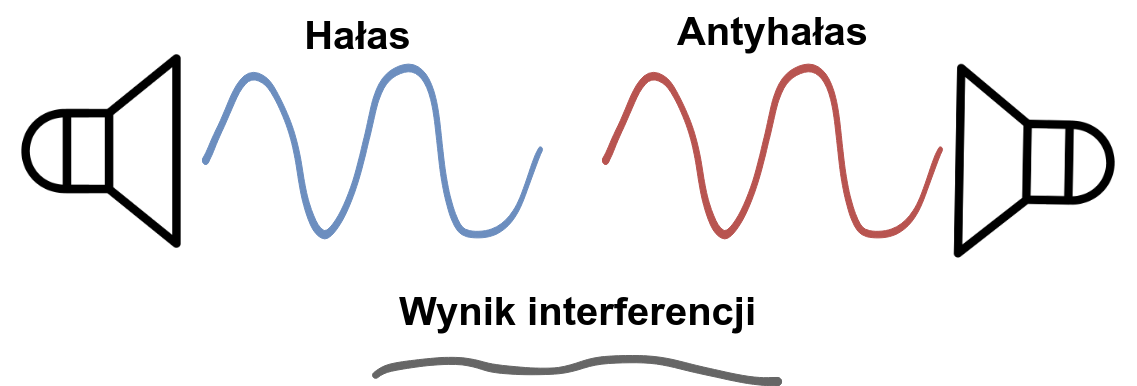
\includegraphics[width=0.63\textwidth]{graf/impl/anc.png}
    \caption{Graficzna wizualizacja idei aktywnej redukcji hałasu}
    \label{intro::anc}
\end{figure}

\par Charakerystyka źródła hałasu w omawianej tematyce jest w większości 
przypadków zmienna w czasie, co powoduje, że częstotliwość, amplituda, faza
jak i prędkość rozchodzenia się drgań w ośrodku jest niestacjonarna.
Takie zachowanie wymaga, żeby projektowany system był adaptacyjny, co oznacza,
że jego zachowanie będzie odpowiednio korygowane, w zależności od zaobserwowanych
zmian charakterystyki źródła. Adaptacja realizowana jedynie w sposób analogowy, 
pomimo że możliwa, posiada duże ograniczenia w zakresie elastyczności i precyzyjności, 
dlatego pożądane jest, aby w systemach tego typu wykorzystać układy cyfrowe,
próbkujące sygnały z czujników oraz przetwarzające je z wykorzystaniem 
odpowiednich algorytmów przetwarzania cyfrowego. 

\section{Zastosowania}
\section{Wymagania, ograniczenia i ocena wydajności}
\subsection{Określenie problematyki}
\subsection{Zakres projektu}
\section{Zwięzła charakterystyka rozdziałów}
